\section{Resultados}
\label{sec:results}

Todos os números desta seção são da fase operacional, sem rótulo no fluxo. A
Tabela~\ref{tab:main} reúne as rodadas principais. ``Env.'' é a fração das instâncias de ataque
pós-aquecimento usadas no treino do modelo adaptativo. O motor MOA não registra essa fração.

\begin{table}[t]
\centering
\caption{Resultados sem vazamento, fase operacional (\%). \modus: hiperparâmetros do artigo para a
base. \modus+ e \modusp: configuração única \texttt{fixed\_q}.}
\label{tab:main}
\setlength{\tabcolsep}{2.6pt}
\begin{tabular}{llrrrrr}
\toprule
Base & Método & Prec. & Rec. & F1 & FPR & Env. \\
\midrule
\multirow{3}{*}{\shortstack[l]{ASEADOS\\(DDoS)}}
 & \modus    &  0,00 &  0,00 &  0,00 &  0,13 & -- \\
 & \modus+   &  0,43 &  0,04 &  0,08 &  2,39 & 99,96 \\
 & \modusp   & 95,19 & 47,07 & \textbf{62,99} &  0,48 & 51,24 \\
\midrule
\multirow{3}{*}{\shortstack[l]{ASEADOS\\(5 classes)}}
 & \modus    &  0,00 &  0,00 &  0,00 &  0,00 & -- \\
 & \modus+   & 77,78 &  0,35 &  0,71 &  0,08 & 99,65 \\
 & \modusp   & 47,83 & 23,09 & \textbf{31,15} & 17,88 & 66,02 \\
\midrule
\multirow{4}{*}{\shortstack[l]{CTU-13\\(C11)}}
 & \modus    & 47,66 & 99,97 & 64,55 & 52,37 & -- \\
 & \modus+   &  0,01 &  0,00 &  0,00 &  3,12 & 100,00 \\
 & \modus+ e congelado & 90,79 & 56,42 & \textbf{69,59} & 2,73 & 43,58 \\
 & \modusp   &  0,06 &  0,00 &  0,01 &  2,60 & 2,41 \\
\midrule
\multirow{3}{*}{\shortstack[l]{Edge-IIoT\\(14 ataques)}}
 & \modus    & 99,79 & 62,23 & 76,66 &  0,12 & -- \\
 & \modus+   & 43,95 &  0,01 &  0,01 &  0,01 & 99,99 \\
 & \modusp   & 96,03 & 86,77 & \textbf{91,17} &  3,14 & 6,90 \\
\bottomrule
\end{tabular}
\end{table}

\subsection{Sem o vazamento, o ataque vira o perfil normal}
\label{sec:poison}
A Figura~\ref{fig:leak} mostra o efeito do vazamento no ASEADOS, com a configuração do artigo. Com
o rótulo no fluxo, todos os fluxos DDoS recebem o mesmo score, acima do piso do limiar, e o F1 é
99,73\%. Sem o rótulo, os mesmos fluxos ficam abaixo do tráfego benigno e nenhum é detectado. A
AUC-ROC do score cai de 100,00\% para 10,70\%: abaixo de 50\%, o detector ordena as classes ao
contrário.

\begin{figure}[t]
\centering
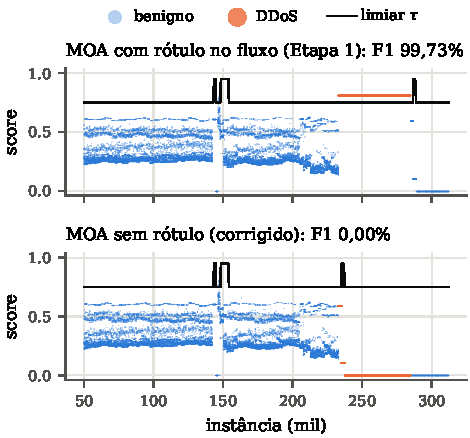
\includegraphics[width=\columnwidth]{leak_aseados}
\caption{ASEADOS, configuração do artigo, fase operacional: score do HST do MOA com o rótulo no
fluxo (acima) e sem ele (abaixo). Benignos amostrados (20 mil).}
\label{fig:leak}
\end{figure}

Normalizar os atributos e acrescentar as taxas (\modus+) não resolve. Nas três bases o \modus+ fica
com F1 abaixo de 1\% (Tabela~\ref{tab:main}), e a medida de envenenamento explica por quê: 99,96\%
dos fluxos DDoS do ASEADOS, 100,00\% dos pacotes de ataque do CTU-13 e 99,99\% dos do Edge-IIoT
treinam o modelo. A AUC-ROC do score é 17,88\%, 0,15\% e 32,87\%, respectivamente. O treino
seletivo falha em cadeia: as primeiras instâncias do ataque ficam abaixo do limiar, treinam o HST,
e as seguintes, iguais a elas, passam a ter massa na referência. No CTU-13, com $W=250$ e um
\emph{flood} de milhares de pacotes por segundo, a referência é substituída dezenas de vezes por
segundo, e o ataque passa a ser o perfil de referência em uma fração de segundo.

O \modus\ original escapa desse efeito em duas bases, mas por um motivo que não é o volume. Sem
normalização, o HST separa por protocolo (Seção~\ref{sec:replication}). No CTU-13 o \emph{flood} é
ICMP, raro no tráfego benigno, e a AUC chega a 99,86\%. No Edge-IIoT, os \emph{floods} ICMP e UDP
têm 100,00\% de alarme, enquanto os \emph{floods} TCP e HTTP têm 0,01\% e 0,02\%
(Tabela~\ref{tab:edge}). É um detector de protocolo raro: acerta quando o ataque usa um protocolo
incomum na rede e erra por completo quando usa o protocolo dominante.

\subsection{ASEADOS: ablação}
A Tabela~\ref{tab:abl} e a Figura~\ref{fig:abl} decompõem o resultado do ASEADOS. Ligadas uma a
uma sobre o \modus+, três das quatro defesas não mudam o F1, que fica abaixo de 0,4\%. O teto de
treino reduz o envenenamento de 99,96\% para 75,21\%, o que ainda é ataque suficiente para dominar
o modelo. Só o modelo congelado detecta algo sozinho (F1 de 16,18\%), e com precisão baixa
(49,30\%). O conjunto completo chega a 62,99\% de F1, com precisão de 95,19\% e 0,48\% de falsos
positivos.

\begin{table}[t]
\centering
\caption{Ablação no ASEADOS (DDoS), fase operacional (\%). ``Aquec.'': instância em que o
aquecimento termina.}
\label{tab:abl}
\setlength{\tabcolsep}{3.5pt}
\begin{tabular}{lrrrrr}
\toprule
Variante & Aquec. & Prec. & F1 & FPR & Env. \\
\midrule
\modus+ (base)             & 50.000 &  0,43 &  0,08 & 2,39 & 99,96 \\
\ + janela de 10\,s        & 50.000 &  2,00 &  0,37 & 2,42 & 99,80 \\
\ + aquecimento adaptativo &  6.651 &  0,96 &  0,05 & 0,53 & 99,97 \\
\ + teto de treino         & 50.000 &  0,67 &  0,12 & 2,38 & 75,21 \\
\ + normalização congelada & 50.000 &  0,81 &  0,15 & 2,43 & 99,92 \\
\ + modelo congelado       & 50.000 & 49,30 & 16,18 & 2,43 & 90,33 \\
\midrule
\modusp\ (todas)           &  6.651 & 95,19 & \textbf{62,99} & 0,48 & 51,24 \\
\ sem janela em tempo      &  6.651 & 93,00 & 62,45 & 0,72 & 51,30 \\
\ sem teto de treino       &  6.651 & 94,67 & 62,88 & 0,54 & 52,93 \\
\ sem aquec. adaptativo    & 50.000 & 54,39 & 19,72 & 2,47 & 74,16 \\
\ sem modelo congelado     &  6.651 &  8,15 &  0,24 & 0,28 & 65,12 \\
\bottomrule
\end{tabular}
\end{table}

\begin{figure}[t]
\centering
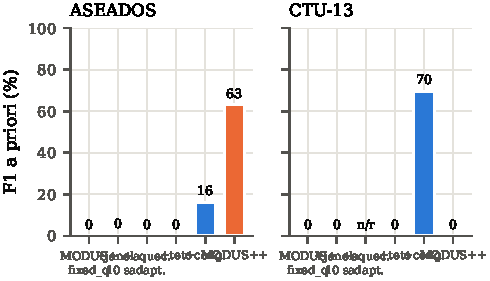
\includegraphics[width=\columnwidth]{ablation}
\caption{F1 a priori por variante. Cada barra azul liga uma defesa sobre o \modus+; a laranja é o
\modusp\ completo. No CTU-13, janela e teto foram avaliados juntos, e o aquecimento adaptativo
sozinho não foi rodado (n/r).}
\label{fig:abl}
\end{figure}

A segunda metade da tabela retira uma peça por vez do \modusp. Sem o modelo congelado o F1 volta a
0,24\%. Sem o aquecimento adaptativo cai para 19,72\%. Sem a janela em tempo ou sem o teto, quase
não muda (62,45\% e 62,88\%). O resultado no ASEADOS vem, portanto, da combinação de duas peças:
o modelo congelado e o aquecimento adaptativo.

A interação entre as duas tem explicação. Com o aquecimento fixo de 50 mil fluxos, o modelo
congelado é treinado com 40 mil e calibrado com 10 mil; o limiar resultante é $\tau_f=0{,}876$, e o
recall é 12,05\%. Com o aquecimento adaptativo, que termina em 6.651 fluxos, o congelado usa 5.320
para treino e 1.331 para calibração, o limiar é $\tau_f=0{,}818$ e o recall sobe para 47,07\%. Os
falsos positivos caem junto, de 2,47\% para 0,48\%. Esse efeito não depende do congelado: ligado
sozinho sobre o \modus+, o aquecimento adaptativo já reduz os falsos positivos de 2,39\% para
0,53\%.

A Figura~\ref{fig:frozen} mostra por que o congelado é a peça decisiva. No modelo adaptativo, a
massa dos fluxos DDoS fica à esquerda da dos benignos: o ataque foi aprendido (AUC de 27,33\%). No
modelo congelado, que nunca viu o ataque, o DDoS fica à direita, com AUC de 94,44\%. O limiar
$\tau_f$, porém, corta a distribuição do ataque ao meio. É por isso que o recall para em 47\%: a
separação existe, mas o quantil 0,999 do aquecimento não cai no vale entre as duas distribuições.

\begin{figure}[t]
\centering
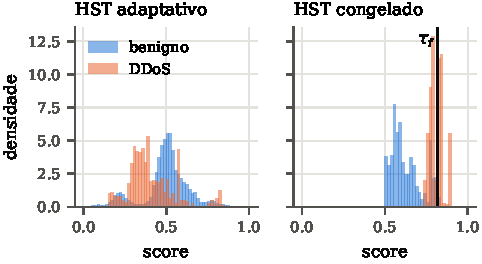
\includegraphics[width=\columnwidth]{frozen_aseados}
\caption{ASEADOS, \modusp: distribuição dos scores pós-aquecimento no HST adaptativo e no HST
congelado. A linha vertical é o limiar $\tau_f$.}
\label{fig:frozen}
\end{figure}

\textbf{Sementes.} Com três sementes do HST, o F1 do \modusp\ é 62,99\%, 68,36\% e 58,86\% (média
de 63,40\%). O \modus+ fica em 0,08\%, 0,18\% e 0,24\%. O ganho não depende da semente, mas a
variação entre sementes, de quase dez pontos, é grande: o limiar congelado vale 0,818, 0,768 e
0,865 nas três rodadas, e a semente 2 troca precisão (81,72\%) por recall (58,75\%).

\subsection{CTU-13: o envenenamento some, o limiar falha}
\label{sec:ctu}
No CTU-13 o resultado a priori do \modusp\ é negativo: F1 de 0,01\%. Os componentes, vistos em
separado, mostram que o método faz o que foi projetado para fazer, e que o erro está em um ponto
específico (Tabela~\ref{tab:ctu} e Figura~\ref{fig:ctu}).

\begin{table}[t]
\centering
\caption{CTU-13, cenário 11, fase operacional (\%). AUC do score do modelo adaptativo. As duas
últimas linhas são análise de sensibilidade, não resultado a priori.}
\label{tab:ctu}
\setlength{\tabcolsep}{3.5pt}
\begin{tabular}{lrrrr}
\toprule
Variante & F1 & FPR & Env. & AUC \\
\midrule
\modus+ (base)              &  0,00 & 3,12 & 100,00 &  0,15 \\
\ + modelo congelado        & 69,59 & 2,73 &  43,58 & 49,78 \\
\ + janela de 10\,s e teto  &  0,00 & 0,04 &   2,07 & 96,47 \\
\modusp\ (todas)            &  0,01 & 2,60 &   2,41 & 72,93 \\
\midrule
\modusp, teto $0{,}1\,c$    & 88,26 & 9,21 &   0,05 & 90,41 \\
\modusp, quantil 0,99       & 83,40 & 5,01 &   0,89 & 92,71 \\
\bottomrule
\end{tabular}
\end{table}

\begin{figure}[t]
\centering
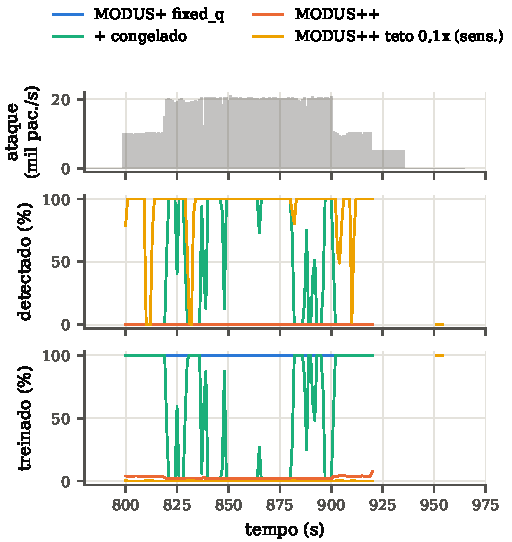
\includegraphics[width=\columnwidth]{ctu_timeline}
\caption{CTU-13, intervalo do \emph{flood}. Acima: pacotes de ataque por segundo. No meio: fração
do ataque detectada. Abaixo: fração do ataque usada no treino do modelo adaptativo.}
\label{fig:ctu}
\end{figure}

\textbf{Janela em tempo e teto eliminam o envenenamento.} Com as duas defesas, a fração do
\emph{flood} que entra no treino cai de 100,00\% para 2,07\%, e a AUC do score adaptativo sobe de
0,15\% para 96,47\%. O teto calculado no aquecimento é de 342 instâncias por segundo por destino,
contra um ataque de 10 a 20 mil pacotes por segundo sobre um único alvo. O modelo deixa de aprender
o ataque e volta a pontuá-lo como anômalo. O F1, porém, continua em 0,00\%, porque o limiar
adaptativo não acompanha: com um limiar fixo escolhido com rótulos, o mesmo score daria F1 de
94,81\%. Esse valor é um teto, não um resultado.

\textbf{O congelado sozinho detecta, mas não protege.} Ligado sobre o \modus+, sem as outras
defesas, o modelo congelado chega a 69,59\% de F1, com precisão de 90,79\% e recall de 56,42\%. A
Figura~\ref{fig:ctu} mostra que a detecção oscila: nos segundos em que o score congelado fica abaixo
de $\tau_f$, o ataque volta a treinar o modelo adaptativo, e 43,58\% do \emph{flood} é aprendido.

\textbf{No conjunto completo, o limiar erra por milésimos.} No \modusp\ o aquecimento adaptativo
termina em 35.318 pacotes, e o congelado é calibrado com $\tau_f=0{,}777$. O score do \emph{flood}
nesse modelo é 0,774. O ataque fica logo abaixo do limiar durante todo o intervalo, e a linha
laranja da Figura~\ref{fig:ctu} não sai do zero. A AUC do congelado é 93,95\%: a separação existe,
como no ASEADOS, e o limiar não a aproveita. As duas rodadas de sensibilidade confirmam a leitura.
Com o quantil 0,99 em vez de 0,999, $\tau_f$ cai para 0,734 e o F1 vai a 83,40\%. Com o teto
dividido por dez, o F1 vai a 88,26\%, ao custo de 9,21\% de falsos positivos. Nenhum dos dois
valores foi escolhido a priori, e não os contamos como resultado do método.

Vale registrar a comparação desfavorável: o \modus\ original, sem normalização, tem F1 de 64,55\%
nesta base com os hiperparâmetros do artigo e de 99,74\% com os hiperparâmetros que o artigo usa no
ASEADOS. Os dois valores vêm da raridade do ICMP, e a diferença entre eles ilustra o peso do
ajuste por base: com a configuração do artigo para o CTU-13, 52,37\% do tráfego benigno gera alarme.

\subsection{Edge-IIoTset e ataques não-DDoS}
\label{sec:edge}
No Edge-IIoTset usamos os 14 tipos de ataque da base (21,1 milhões de quadros, 9,87 milhões de
ataque). É o melhor resultado do \modusp: F1 de 91,17\%, com precisão de 96,03\% e recall de
86,77\%, contra 76,66\% do \modus\ original e 0,01\% do \modus+. O envenenamento cai de 99,99\%
para 6,90\%, e a AUC do score adaptativo vai de 32,87\% para 91,95\%. O aquecimento adaptativo
termina no mínimo permitido, 5.000 quadros.

\begin{table}[t]
\centering
\caption{Edge-IIoTset: taxa de alarme por classe na fase operacional (\%). $n$ em milhares de
quadros (no \modusp, 11.254 mil normais, pois o aquecimento é mais curto).}
\label{tab:edge}
\setlength{\tabcolsep}{4pt}
\begin{tabular}{lrrrr}
\toprule
Classe & $n$ & \modus & \modus+ & \modusp \\
\midrule
DDoS ICMP             &  2.914 & 100,00 & 0,00 & 99,88 \\
DDoS UDP              &  3.216 & 100,00 & 0,00 & 99,72 \\
DDoS TCP              &  2.020 &   0,01 & 0,00 & 97,14 \\
DDoS HTTP             &    229 &   0,02 & 0,05 & 68,32 \\
\midrule
Vulnerability scanner &    266 &   0,13 & 0,09 & 77,75 \\
Ransomware            &     11 &  11,19 & 0,08 & 43,30 \\
Fingerprinting        &      1 &  69,22 & 0,00 & 34,86 \\
MITM                  &      1 &  66,80 & 3,91 & 18,31 \\
SQL injection         &     51 &   0,11 & 0,00 & 16,45 \\
Backdoor              &     25 &   3,32 & 0,01 & 12,92 \\
Password              &  1.054 &   0,17 & 0,00 &  9,05 \\
Uploading             &     38 &   0,16 & 0,06 &  8,25 \\
Port scanning         &     23 &  11,40 & 0,05 &  5,88 \\
XSS                   &     16 &   4,55 & 0,00 &  4,30 \\
\midrule
Normal (falso alarme) & 11.209 &   0,12 & 0,01 &  3,14 \\
\bottomrule
\end{tabular}
\end{table}

A Tabela~\ref{tab:edge} detalha por classe. O ganho sobre o \modus\ original está nos
\emph{floods} que usam o protocolo dominante da rede: o DDoS TCP vai de 0,01\% para 97,14\% de
alarme, e o DDoS HTTP, de 0,02\% para 68,32\%. Os \emph{floods} ICMP e UDP continuam acima de
99,7\%. O custo é o falso alarme no tráfego normal, que sobe de 0,12\% para 3,14\%.

Fora dos DDoS, o resultado é fraco. Só o \emph{Vulnerability scanner} passa de 50\% de alarme. Sete
das dez classes não-DDoS ficam abaixo de 20\%, e \emph{Password}, a mais volumosa delas, tem
9,05\%, pouco acima da taxa de falso alarme. Em quatro classes pequenas (\emph{Fingerprinting},
MITM, \emph{Port scanning} e XSS), o \modus\ original tem taxa maior que a do \modusp. Os atributos usados (portas, protocolo,
tamanho e taxas) descrevem volume e cabeçalho, e não o conteúdo que caracteriza esses ataques. O
F1 alto no Edge-IIoT vem dos DDoS, que são 85\% das instâncias de ataque.

O ASEADOS com as cinco classes mostra o outro lado do modelo congelado. O \modusp\ sobe de 0,71\%
para 31,15\% de F1 e detecta 100,00\% do \emph{Probe}, mas apenas 38,82\% do DDoS, 22,90\% do
\emph{Bot} e 10,95\% do DoS, com 17,88\% de falsos positivos. Nessa variante há ataques
desde o início do fluxo: os primeiros 50 mil fluxos contêm 20.711 deles. O modelo congelado
depende de um aquecimento limpo, e a AUC do seu score aqui é 50,05\%, igual ao acaso.

\subsection{Sensibilidade}
\label{sec:sens}
Os parâmetros novos foram fixados antes das rodadas. Variamos três deles depois, para medir o quanto
o resultado depende dessas escolhas (Tabela~\ref{tab:sens}).

\begin{table}[t]
\centering
\caption{Sensibilidade do \modusp\ aos parâmetros novos (\%). A primeira linha de cada base é a
configuração a priori.}
\label{tab:sens}
\setlength{\tabcolsep}{3pt}
\begin{tabular}{llrrrr}
\toprule
Base & Variação & Prec. & Rec. & F1 & FPR \\
\midrule
\multirow{4}{*}{ASEADOS}
 & a priori ($T=10$\,s; $q=0{,}999$) & 95,19 & 47,07 & 62,99 & 0,48 \\
 & $T=1$\,s        & 99,01 &  9,88 & 17,97 & 0,02 \\
 & $T=60$\,s       & 93,85 & 47,19 & 62,80 & 0,63 \\
 & $q=0{,}99$      & 81,69 & 48,83 & 61,12 & 2,22 \\
\midrule
\multirow{3}{*}{CTU-13}
 & a priori ($c$; $q=0{,}999$)       &  0,06 &  0,00 &  0,01 & 2,60 \\
 & teto $0{,}1\,c$ & 82,96 & 94,29 & 88,26 & 9,21 \\
 & $q=0{,}99$      & 88,24 & 79,07 & 83,40 & 5,01 \\
\bottomrule
\end{tabular}
\end{table}

No ASEADOS o método é estável para janelas de 10 e 60 segundos e para o quantil do limiar
congelado. A janela de 1 segundo degrada o resultado (F1 de 17,97\%): com ela o aquecimento
adaptativo termina em outro ponto (12.025 fluxos), o limiar congelado sobe para $\tau_f=0{,}854$ e
o recall cai para 9,88\%. Uma explicação provável é que, na taxa baixa desta base, janelas de
1 segundo raramente juntam as 50 instâncias exigidas para a troca. No CTU-13 a sensibilidade é extrema, pelo motivo já visto: qualquer variação que
mova o limiar ou o score em poucos milésimos leva o F1 de 0\% para mais de 80\%. Um resultado que
muda tanto com uma casa decimal de um quantil não deve ser lido nem como fracasso nem como sucesso
do modelo, e sim como evidência de que a regra de limiar é o elo fraco.

\subsection{Custo computacional}
O \modusp\ mantém dois HST e pontua cada instância nos dois. Ainda assim o motor em \texttt{numpy}
processou o CTU-13 (6,3 milhões de pacotes) em 1.294\,s e o Edge-IIoTset (21,1 milhões de quadros)
em 1.384\,s, cerca de 4,9 mil e 15,3 mil instâncias por segundo. O ganho vem do cálculo em lote: o
score de uma janela inteira é calculado de uma vez, porque a referência não muda entre trocas. Os
tempos são indicativos, pois várias rodadas dividiram a mesma máquina. Para o mesmo fluxo do
Edge-IIoTset, o artigo original reporta 14.893\,s.
